	\subsection{Теоретические исследования}
	\label{theoreticalOverview}
		\hspace{1em}
		Процесс взаимодействия частиц с несущей фазой очень хорошо описан в книге \cite{Richardson}. Данная книга предоставляет в явном виде решение большого количества инженерных задач, связанных с течениями дисперсных сред. В конечном виде эти решения являются в большой степени приближёнными, применимы в ограниченном числе случаев и описывают, в основном, общие параметры системы, не давая информации о структуре течения несущей фазы, фокусируясь именно на описании частиц. Тем не менее, теоретические модели, сформулированные в этой книге охватывают широкий диапазон физических процессов, связанных с течениями жидкостей с дисперсными включениями, и могут быть крайне полезны для математического описания таких течений.
		\subsubsection*{Степень очистки}
		\addcontentsline{toc}{subsubsection}{Степень очистки}
		Диргоу и Лейт \cite{DirgoLeith} в своей статье систематизировали теоретические модели, применяемые для расчётов рабочих параметров системы, выделив три основных подхода к описанию циклонов.
			\subparagraph{I. Подход, основанный на времени полёта частиц\\}
			Допустим, частица попадает в циклон на определённом расстоянии от оси фильтра. Частица должна переместиться из этого положения к стенке для того, чтобы быть отфильтрованной. Критический диаметр частицы это такой диаметр, при котором частица перемещается ровно на это расстояние за время пребывания в циклоне. Различные заключения о начальном положении частицы и времени пребывания приводят к различным приближённым решениям. Теория Лэппла \cite{Lapple} является наиболее часто используемым примером такого подхода. Предположим, что пыль, поступающая в циклон, равномерно распределена по всему входному сечению. Лэппл определил критический диаметр частиц для циклонов как диаметр, при котором, частицы, перемещаясь от середины входного сечения до стенки, за время пребывания в циклоне фильтруются с 50\% эффективностью:
			\begin{equation}
				\label{LappleEquation}
				d_{50} = \sqrt{\frac{9\mu b}{2 \pi \rho_p U_i C_d N_t}},
			\end{equation}
			где $\rho_p$ - плотность частиц, $U_i$ - скорость газа на входе в циклон, $\mu$ - динамическая вязкость воздуха, $b$ - ширина входного сечения фильтра, $C_d$ - коэффициент сопротивления.
			
	Число оборотов $N_t$, которые совершает газ внутри фильтра, может быть рассчитано по формуле $N_t = tU_i/\pi D$, а время пребывания $t$ равно отношению объёма циклона к объёмному расходу воздуха $Q$ \cite{Kuo}.
	
	Эффективность для частицы произвольного диаметра $d$ может быть определена из величины отношения этого диаметра к $d_{50}$.
	\begin{figure}[ht]
		\centering
		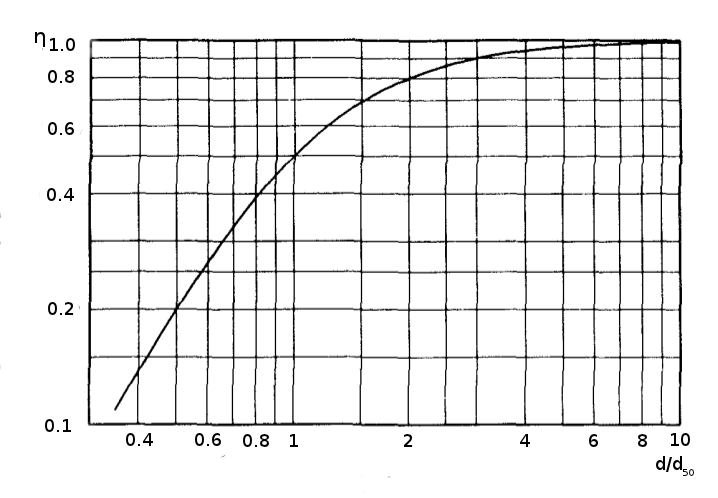
\includegraphics[scale=0.5]{Lapple}
		\caption{Степень очистки в зависимости от $d/d_{50}$}
		\label{fig:lapple}
	\end{figure}
	На \textit{рисунке \ref{fig:lapple}} показана степень очистки в зависимости от $d/d_{50}$, построенная на основе экспериментов Лэппла. Теодоре и де Паола \cite{Theodore} предлагают для определения степени очистки воздуха использовать следующее соотношение, определённое на основе экспериментов Лэппла:
			\begin{equation}
				\eta = \frac{1}{1 + (d/d_{50})^{-2}}
			\end{equation}
			\subparagraph{II. Подход, основанный на статике частиц\\}
			При таком подходе критический диаметр определяется как диаметр частицы, при котором действующая на частицу центробежная сила полностью компенсируется силой сопротивления. Такие частицы должны бесконечно вращаться вокруг границы ядра фильтра, расположенного под выходным сечением. Сила сопротивления, действующая на более мелкие частицы превышает центробежную силу так, что такие частицы пересекают эту границу и, поднимаясь наверх, вылетают из циклона. Более крупные частицы относятся к стенкам циклона и могут, таким образом, быть отфильтрованы. При таком определении критического диаметра, степень фильтрации растёт от нуля для частиц меньше критического диаметра до единицы для частиц, диаметром больше критического. На практике такое строгое разделение недостижимо из-за флуктуаций скорости, а эффективность для критического диаметра, в среднем, должна быть равной 50\%.
			
			Примером этого подхода может служить теория, предложенная в статье Барта \cite{Barth}. Барт определил границы ядра циклона, как воображаемое продолжение стенок выходной трубы до нижнего сечения фильтра или стенок конуса. При таком определении границы, критическая скорость для осаждения статических частиц выражается формулой
			\begin{equation}
				U^{*}_{ts} = \frac{Qg}{2 \pi h^{*} U^2_t}
			\end{equation}
			Степень очистки для других диаметров частиц определяется через отношение критической скорости произвольных частиц к критической скорости статических частиц
			\begin{equation}
				\frac{U_{ts}}{U^{*}_{ts}} = \frac{\pi h^{*}U^2_t\rho_p d^2}{9 \mu Q},
			\end{equation}
			где $h^{*}$ - высота ядра циклона, которая может быть найдена из геометрических соображений, а $Q$ - расход воздуха через входное сечение фильтра. Тангенциальная скорость газа на границе ядра, определяется, как 
			\begin{equation}
				U_t = U_o\left(\frac{(D_e/2)(D-b)\pi}{2ab\alpha + h^{*}(D-b)\lambda \pi}\right),
			\end{equation}
			где $\lambda = 0.02$ - коэффициент трения, $\alpha = 1-1.2(b/D)$, $U_o$ - скорость газа в выходном сечении, $a$ и $b$ - соответственно, высота и ширина входного сечения \cite{Barth}.
			\begin{figure}[ht]
				\centering
				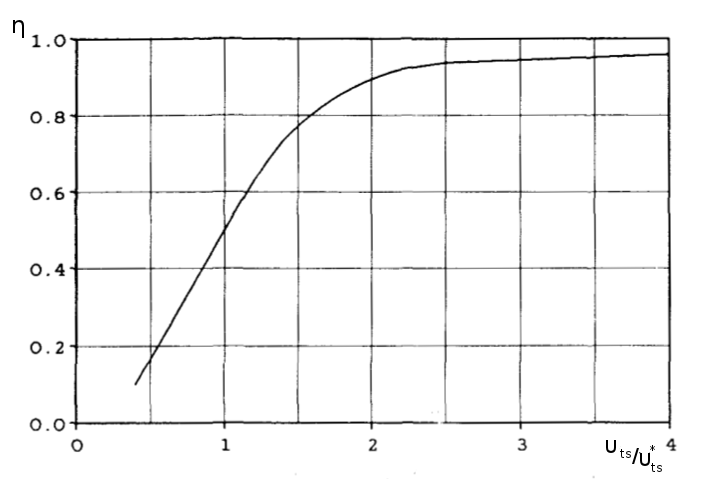
\includegraphics[scale=0.48]{Barth}
				\caption{Степень очистки в зависимости от $U_{ts}/U^{*}_{ts}$}
				\label{fig:barth}
			\end{figure}
			На \textit{рисунке \ref{fig:barth}} показана зависимость степени очистки от $U_{ts}/U^{*}_{ts}$, построенная Бартом на основе экспериментальных результатов для нескольких конфигураций циклона. Кривая Барта хорошо аппроксимируется выражением
			\begin{equation}
				\eta = \frac{1}{1+ (U_{ts}/U^{*}_{ts})^{-3.2}}
			\end{equation}
	
			\subparagraph{III. Прямой расчёт эффективности очистки\\}

			Последний подход позволяет рассчитать эффективность очистки для любого размера частиц и любой конфигурации циклонов. Кривая степени очистки может быть определена без использования обобщённых кривых, основанных на критическом диаметре. Примерами такого подхода являются теория Лейта-Лихта \cite{LeithLicht} и теория Диетца \cite{Dietz}.
			
			Течение в промышленных циклонах на практике всегда является турбулентным. Модель Лейта-Лихта учитывает влияние турбулентности предполагая, что на любой высоте внутри циклона неосевшая пыль представляет собой равномерную смесь. Среднее время пребывания в циклоне определяется на основе его геометрических размеров и расходе воздуха. Итоговое выражение для степени очистки циклона выглядит следующим образом:
			\begin{equation}
				\eta = 1 - \exp[-2 (C\Psi)^{1/(2n+2)}].
			\end{equation}
			Влияние свойств частиц и газа учитывается в модифицированном инерционном параметре $\Psi$.
			\begin{equation}
				\Psi = \frac{\rho_p d^2 U_i (n+1)}{18 \mu D}.
			\end{equation}
			Здесь $C$ - безразмерный геометрический параметр, который зависит только от конфигурации фильтра:
			\begin{equation}
				\begin{aligned}
					\label{geometricParameterEfficiency}
					&C = \frac{\pi D^2}{ab} \Bigg[ 2 \left\lbrace 1 - \left( \frac{D_e}{D}\right)^2 \right\rbrace\left( \frac{h_e}{D} - \frac{a}{2D} \right) + \\ &+ \frac{1}{3} \left( \frac{h_e + l - h}{D} \right)\left( 1+\frac{d_c}{D} + \frac{d_c^2}{D^2}  \right) + \frac{h}{D} - \left( \frac{D_e}{D} \right)^2\frac{l}{D} - \frac{h_e}{D}\Bigg]			
				\end{aligned}
			\end{equation}
			Истинная длина циклона, $l$ определяется как максимальное расстояние, которое преодолевает вращающийся поток в зоне под выходной трубой. 
			\begin{equation}
				\label{naturalLength}
				l = 2.3D_e\left(\frac{D^2}{ab}\right)^{1/3}.
			\end{equation}
			Диаметр конуса на истинной длине определяется, как
			\begin{equation}
			\label{diameterAtNaturalLength}
				d_c = D - \frac{(D-B)(h_e + l -h)}{H - h}
			\end{equation}
			Если истинная длина превышает $(H-h_e)$, $l$ в уравнениях (\ref{geometricParameterEfficiency}) и (\ref{diameterAtNaturalLength}) заменяется на $(H - h_e)$.
			
			Степень экспоненты, $n = 0.5 \div 0.9$, определяет изменение тангенциальной скорости в радиальном направлении: $U_tr^n = const$. Эмпирическая формула для определения $n$ при произвольном диаметре циклона и заданной температуре газа выглядит следующим образом \cite{Alexander}:
			\begin{equation}
				\label{incrementN}
				n = 1 - \left[ (1-0.67D^{0.14})(T/283)^{0.3} \right]
			\end{equation}
			
			Модель Диетца \cite{Dietz} является модифицированным вариантом модели Лейта-Лихта. Диетц разделяет циклон на три региона -- входной участок, область опускающегося течения и ядро циклона. Предполагается, что под действием турбулентности устанавливается равномерный в радиальном направлении профиль концентрации неотфильтрованных частиц внутри каждого региона. Предполагается также, что происходит обмен частицами между областью опускающегося течения и ядром циклона. Для расчёта эффективности циклона предлагается формула
			\begin{equation}
				\eta = 1 - \left[ K_0 - \sqrt{K_1^2 + K_2^2} \right]\exp{\left[\frac{-\pi (2h_e - a)\rho_p d^2 U_i}{18 \mu ab}\right]},
			\end{equation}
			где 
			\begin{eqnarray}
				K_0 &=& \frac{1}{2}\left[ 1 + \left(\frac{D_e}{D}\right)^{2n}\left(1+\frac{9\mu ab}{ \pi \rho_p l d^2 U_i}\right) \right] \\
				K_1 &=& \frac{1}{2}\left[ 1 - \left(\frac{D_e}{D}\right)^{2n}\left(1+\frac{9\mu ab}{ \pi \rho_p l d^2 U_i}\right) \right] \\
				K_2 &=& \left(\frac{D_e}{D}\right)^{2n}.
			\end{eqnarray}
			Как и в модели Лейта-Лихта, $l$ должна быть заменена на $(H-h_e)$, если $l>(H-h_e)$. Величина $n$ может быть вычислена по формуле (\ref{incrementN}).
	\subsubsection*{Перепад давления}
	\addcontentsline{toc}{subsubsection}{Перепад давления}
		Величина перепада давления, создаваемого циклоном, являясь показателем необратимых потерь энергии, имеет чрезвычайно важное значение, поскольку она непосредственно связана с эксплуатационными расходами. Перепад давления определяется, как разница давлений между входным и выходным сечениями фильтра \cite{Utikar}. Циклоны в этом плане имеют одну важную особенность, которая заключается в наличии радиальной компоненты скорости в выходном сечении фильтра, которая затрудняет определение статического давления в этой области. На практике, разница давлений между входной и выходной границей ниже, чем истинный перепад давления.
		
		Обобщенный вариант формулы для определения давления представляет собой произведение числа Эйлера на скоростной напор:
		\begin{equation}
			\triangle P_{air-only}  = \frac{16ab}{D_e^2} \left( \frac{\rho_g U_i^2}{2} \right).
		\end{equation}
		Для слабо запылённых потоков уравнение записанное с использованием безразмерных геометрических параметров, предложенное Лэпплом является более надёжным:
		\begin{equation}
			\triangle P_{air-only} = \frac{16\left(\frac{a}{D}\right)\left(\frac{b}{D}\right)}{\left(\frac{D_e}{D}\right)^2} \frac{\rho_g U_i^2}{2} = \frac{16\left(\frac{a}{D}\right)\left(\frac{b}{D}\right)}{\left(\frac{D_e}{D}\right)^2}\left(\frac{\rho_g\left(\frac{Q}{ab}\right)^2}{2}\right).
		\end{equation}
		Примечательно, что перепад давления сначала падает с увеличением концентрации дисперсных включений, а потом снова начинает расти, начиная с некоторой, достаточно большой, концентрации примесей \cite{Shrikant}. Для определения перепада давления с учётом концентрации примеси используется уравнение Смольника \cite{Smolik}
		\begin{equation}
			\triangle P_{with-solids} = \triangle P_{air-only} (1-0.02c^{0.6}),
		\end{equation}
		где $c$ - концентрация твёрдых частиц на входе в циклон.